% Plantilla para realizar informes en LaTeX para los
% laboratorios dirigidos por el profesor Luis Torres. 
% Ago 2016.

\documentclass[letterpaper,12pt, twocolumn]{article}
\usepackage[spanish]{babel} % nombre de secciones automáticas en español. 
\usepackage[utf8]{inputenc}
\usepackage[T1]{fontenc}
\usepackage{lmodern}

%page margins
\usepackage[left=2cm,top=2cm,right=2cm,bottom=2cm]{geometry}
\usepackage{balance} %balance the columns in the last page
  
\usepackage{graphicx} % insert graphics jpg, png.
\usepackage[table]{xcolor} %color, also in tables
\usepackage{amsmath, amssymb, amsfonts} %math symbols
\usepackage[small]{titlesec} % section titles small

% Añade tus paquetes aquí
%\usepackage{...}


% Plantilla de titulo, logo, etc. Redefinimos \maketitle
\newcommand{\asignatura}[1]{\def\asignaturaVal{#1}}
\newcommand{\titulo}[1]{\def\tituloVal{#1}}
\newcommand{\grupoLab}[1]{\def\grupoLabVal{#1}}
\newcommand{\autores}[1]{\def\autoresVal{#1}}
\newcommand{\uninorteEmails}[1]{\def\uninorteEmailsVal{#1}}
%
\makeatletter         
\def\@maketitle{
    \raggedright
    
\includegraphics[width = 18mm]{figs/un_logo.jpg} \parbox[b]{0.8\textwidth}{\large \textbf{División de Ingenierías \\ Dept. de Ingenierías Eléctrica y Electrónica} \\ \asignaturaVal. \\ Docente: Jorge Martínez} \\[4ex]
    \begin{center}
        {\LARGE \bfseries \tituloVal }\\[0ex] 
        {\normalsize Grupo \grupoLabVal: \autoresVal}\\[0ex] 
        {\normalsize \texttt{\{\uninorteEmailsVal\}@uninorte.edu.co}} \\[0ex] 
        {\bfseries \today}\\[4ex]
    \end{center}}
\makeatother


%Encabezado de reporte: Edite con su información.
\asignatura      {Procesamiento Digital de Imágenes IEN 8450 }
\grupoLab        {1}
\autores         {Jorge Aguilar, Jorge Díaz, Jorge Lambraño}
\uninorteEmails  {jdaguilar, eduranj, jelambrano}
\titulo          {Intérprete de imágenes digitales de partituras}


\begin{document}
\maketitle %genera el titulo, autores, emails, etc. 



\begin{abstract}
En el siguiente informe se presentará la propuesta para el 
proyecto final de la materia Procesamiento Digital de 
Imágenes, además de su justificación y los objetivos a 
alcanzar con el proyecto.  
\end{abstract}

\section{Introducción}
La visión por computadora ha sido una de las áreas 
de la informática de más rápido desarrollo, esto se 
debe a que puede ser aplicada en múltiples contextos 
y es, en mucho casos, la herramienta más apropiada 
para solución de problemas. Lo que hace fascinante a 
la visión por computadora es el hecho que puede 
aplicarse en múltiples plataformas, ya sea desde 
computadores con diferentes sistemas operativos, 
teléfonos inteligentes o sistemas empotrados en 
dispositivos mucho menos potentes. \\

Por otra parte, en el estudio de la música se 
presentan dificultades para interpretar una partitura, 
ya sea porque es muy extensa o porque tiene demasiadas
figuras musicales. Cuando existe un audio de dicha 
partitura la comprensión y posterior interpretación 
se facilita. Sin embargo, es muy probable que ciertas 
partituras no tengan un audio que las complemente, 
sobretodo cuando son de canciones recientes o no tan 
famosas. Si el estudiante de música tuviese una 
herramienta que permitiera reproducir cualquier 
pentagrama tendría una herramienta de estudio muy útil. \\

Por esta razón se diseñará a través de visión por 
computadora, una herramienta que brinde solución a 
esta problemática, es decir, que sea capaz de extraer 
la información de una partitura y a partir de ésta 
generar una melodía. Se utilizará visión por 
computadora puesto que es necesario procesar la imagen 
de una partitura. Ya que para esta aplicación, ésta es 
la mejor forma de adquisición de datos. 

\section{Objetivos}

\subsubsection*{Objetivo General}
Interpretar la melodía de una partitura digitalizada 
aplicando vision por computadora y posteriormente 
generar archivos musicales y de audio en formatos que 
pueda repoducirse. 

\subsubsection*{Objetivos Específicos}
\begin{enumerate}

\item[•] Reconocer de la imagen de un pentagrama las 
diferentes figuras (tiempos) y su posición (notas). 

\item[•] Generar un archivo que guarde la información del 
pentagrama a partir de las figuras reconocidas.

\item[•] Convertir el archivo anterior en una melodía. 

\end{enumerate}

\section{Justificación}

Se puede entender la música como un lenguaje y este 
proyecto permite la unión de este lenguaje con la 
visión por computadora. Desde este punto de vista, 
este sistema traduce de lo “escrito” a lo “hablado”, 
donde el contenido del mensaje es una melodía. \\

Hay muchos casos donde esta traducción puede llegar 
a ser necesaria, para una persona incapaz de leer la 
partitura, ya sea  por falta de conocimientos o por 
alguna discapacidad visual. Esta aplicación brinda la 
oportuniddad de adquirir la información que está dentro 
de dicha partitura. 

\section{Procedimiento}

El procedimiento consiste en primer lugar leer una 
partitura digitalizada, ya sea por software, por escaneo 
o por foto. Por medio de un programa escrito en 
\textbf{python}, 
y apoyándonos en sus librerías, especialmente en la 
librería \textbf{opencv}, poder leer la imagen, 
aplicarle un 
proceso de binarización y un proceso de detección de 
bordes. Esto con el fin de obtener las diferentes 
líneas o figuras que puede tener un pentagrama. 
Luego, aplicando un proceso de correlación determinar 
cada figura detectada, por ejemplo: Detectar si una 
figura es una corchea o semicorchea. El la Figura 
\ref{bloques} se observan los elementos que conforman 
este proyecto. 

\begin{figure}[h]
\centering
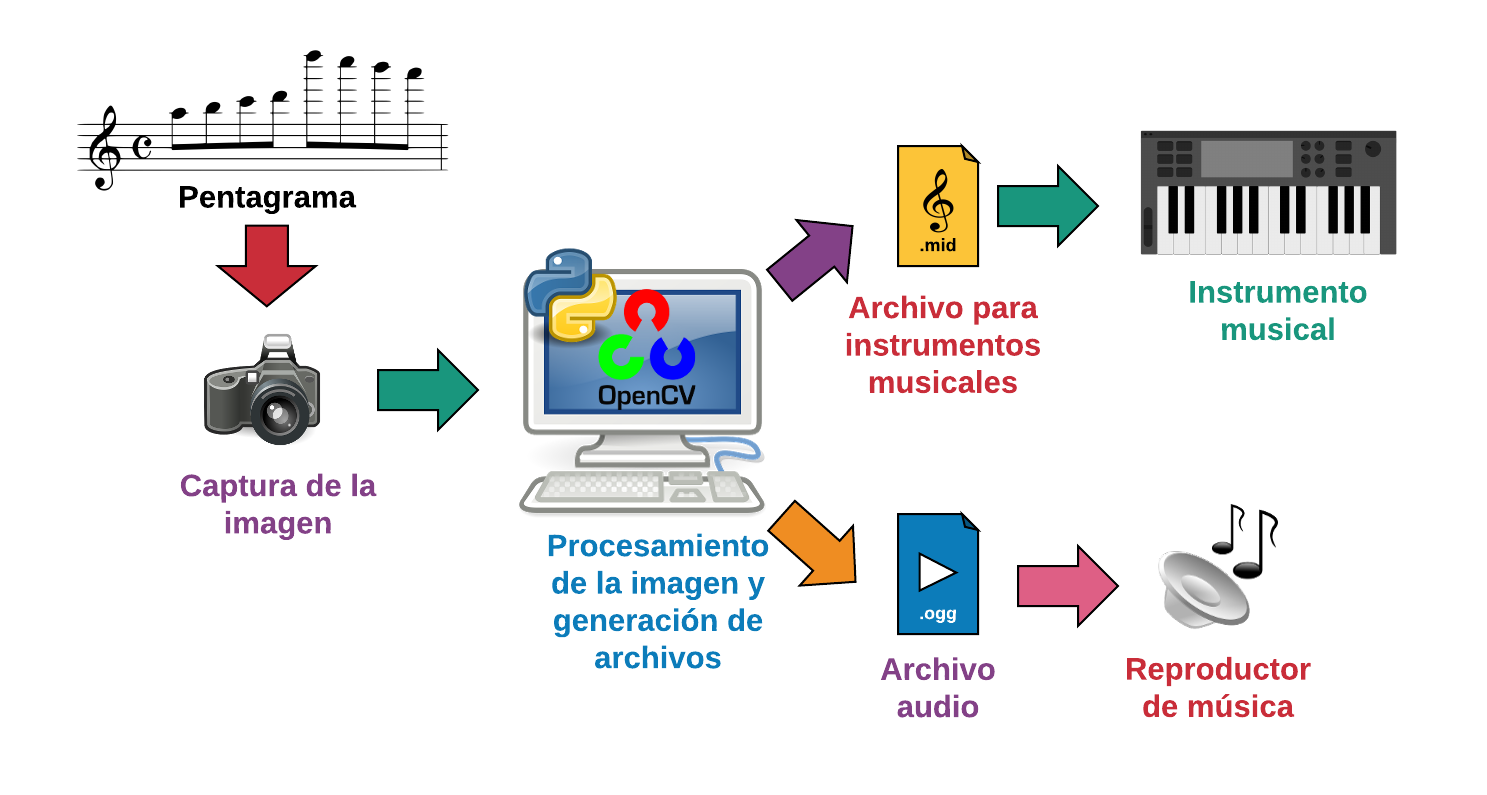
\includegraphics[clip,width=\columnwidth]
{figs/bloques.png}
\caption{Diagrama de bloques de los elementos 
que conforman al proyecto final.}
\label{bloques}
\end{figure}

Cuando tengamos todas las figuras detectadas, el 
algoritmo detectará el orden en que estas aparecen 
en el pentagrama, este es un procedimiento importante 
a la hora de construir la melodía. Para construir la 
melodía, se construirá cada tono dependiendo de la 
posición de la figura en el pentagrama y el tiempo 
lo determina la figura. Los tonos se construirán 
asociando la frecuencia de sonido respectiva.

\section{Resultados Esperados}
Se espera que la eficiencia de este algoritmo sea alta 
(por encima del 80\%), ya que así como en los números, 
en la música un cambio de figura o de nota puede alterar 
gravemente la melodía. Por este motivo se diseñará un 
sistema de reconocimiento óptico musical (OMR) cuya 
eficiencia sea la más alta posible. \\

El sistema arroja dos archivos uno con extensión .mid 
y otro en un formato de audio: .mp3, .wma, .wav o .ogg.
Se espera que no sólamente el sistema sea capaz de 
extraer la melodía, además los archivos que se generan 
se puedan abrir en otras plataformas, como un instrumento 
musical en el caso del archivo .mid o en un reproductor 
de audio para el archivo .ogg. 

\section{Conclusiones}

Se puede concluir que la visión por computadora puede 
utilizarse para la interpretación de símbolos musicales, 
sin embargo el procesamiento que se le debe realizar 
a las imágenes es relativamente complejo. Una vez 
obtenida la información del pentagrama se busca 
guardarla en archivos para que el procesamiento 
no tenga que hacerse nuevamente, estos archivos 
pueden ser ejecutados en un reproductor musical o en 
instrumento. Finalmente, se busca que el algoritmo 
reconozca las imágenes con un alto nivel de eficiencia, 
puesto que en la música se necesita precisión. 

\end{document}
